\documentclass [12pt, a4paper] {article}
\usepackage[utf8x]{inputenc}
\usepackage[english,russian]{babel}
\usepackage[T2A]{fontenc}
\usepackage {graphicx}

\begin {document}

\thispagestyle {empty}

\begin {center}
    \ \vspace{-4cm}

    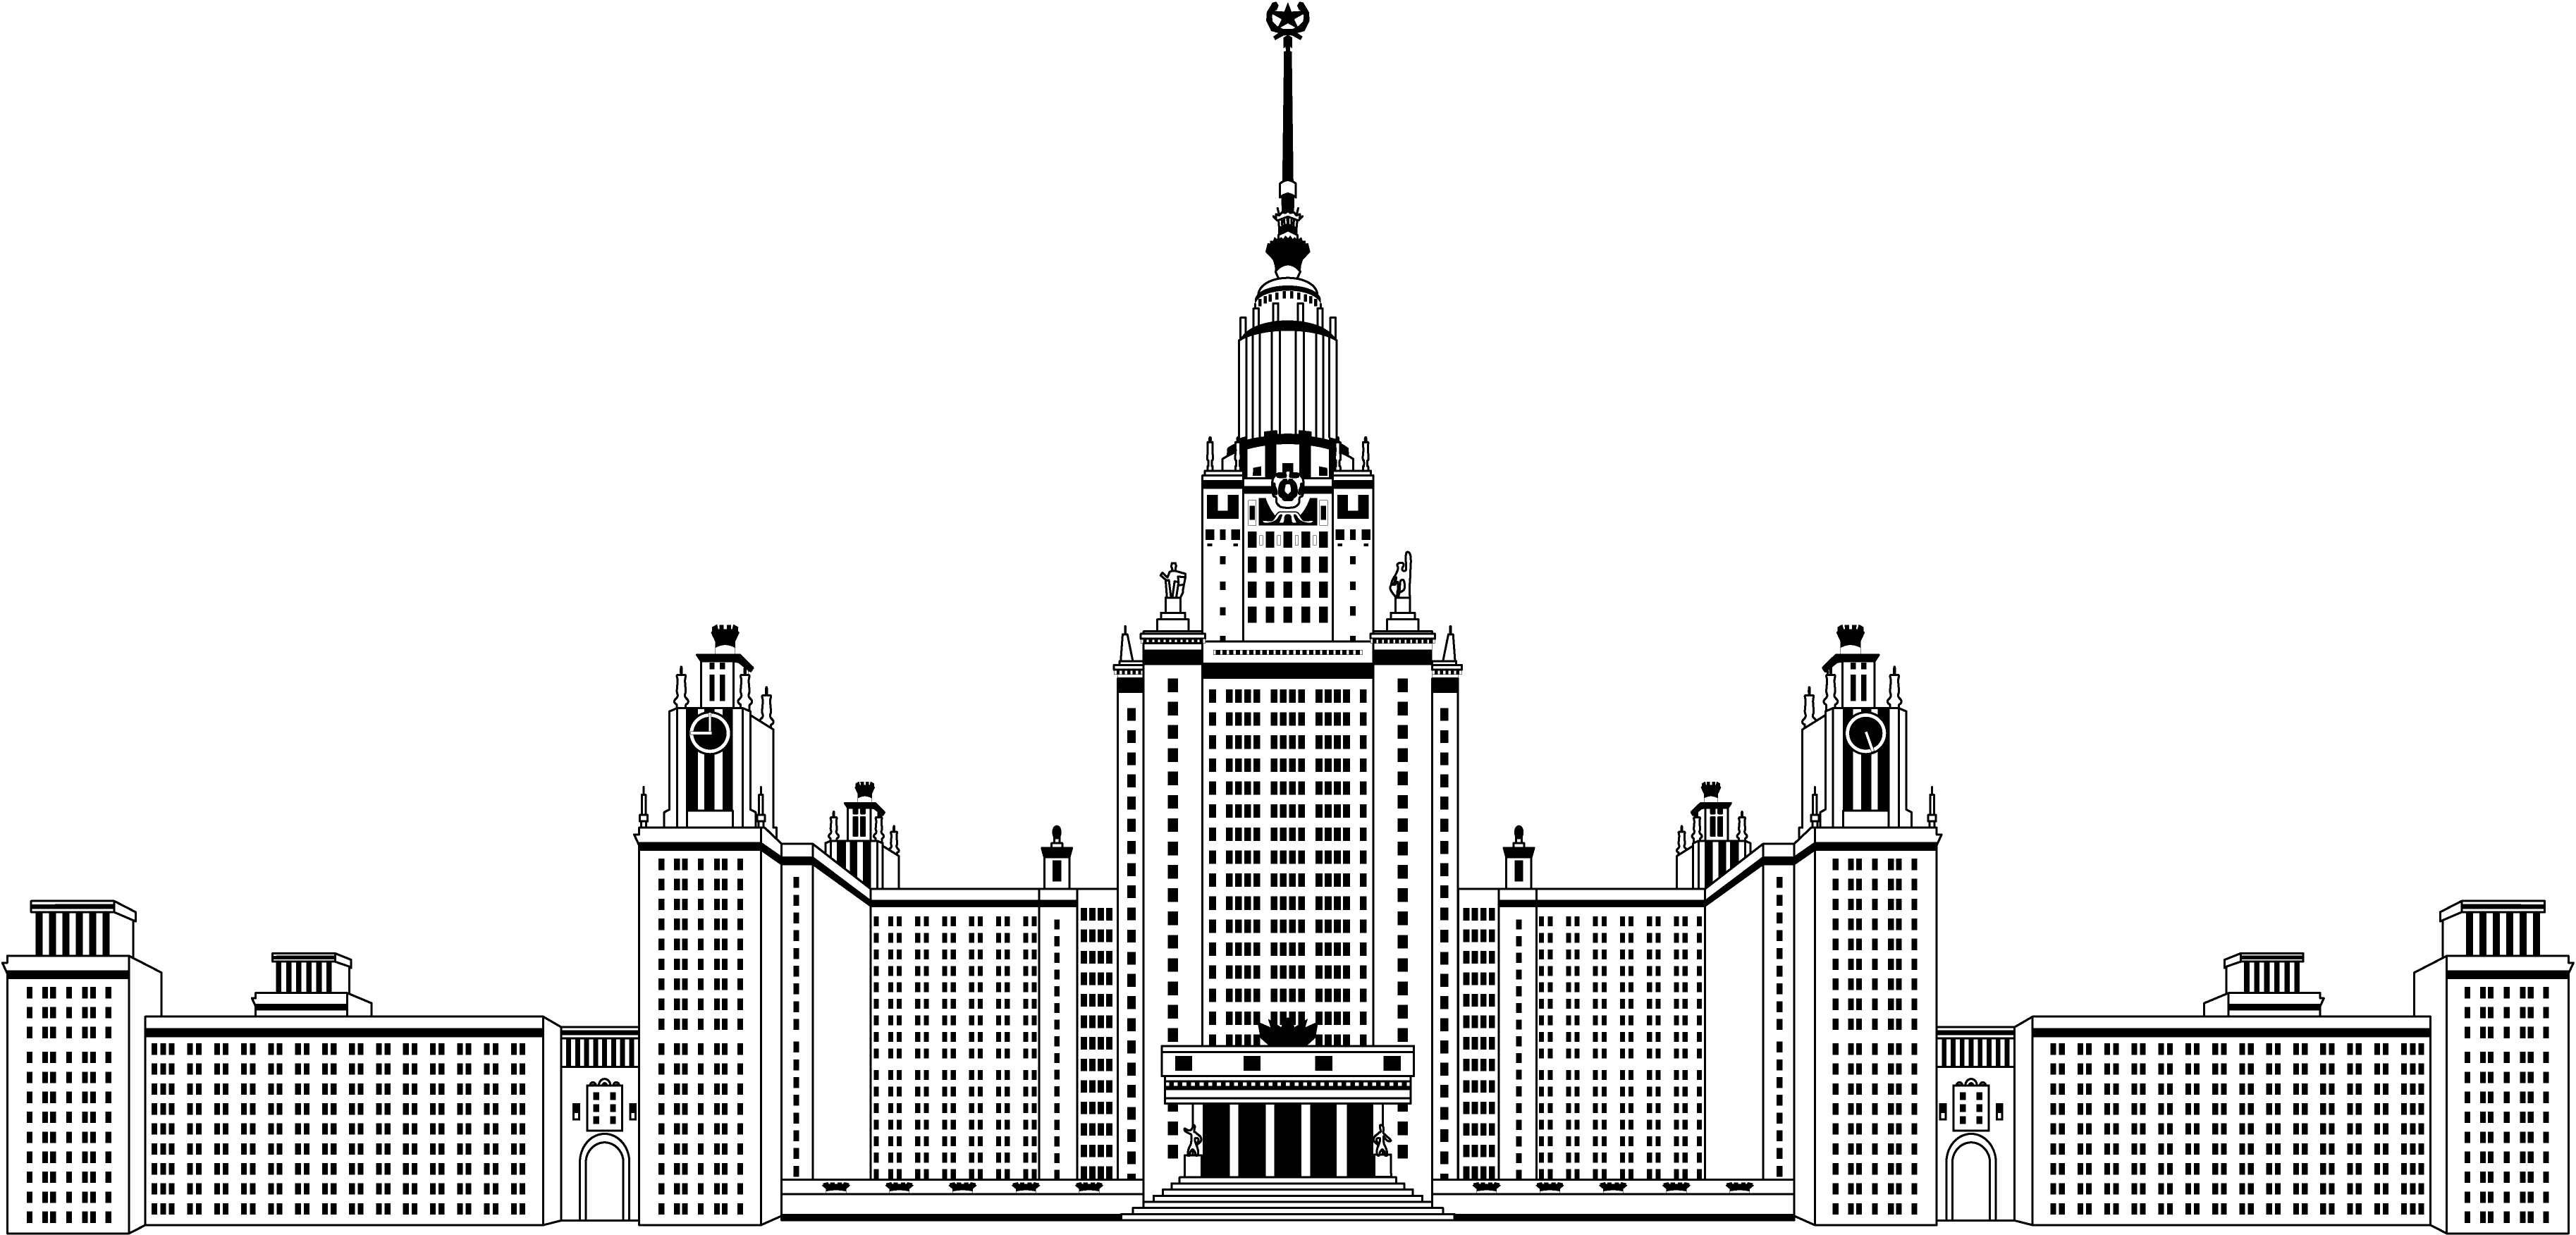
\includegraphics [width = 0.5 \textwidth] {msu.png} \\
    {\scshape Московский Государственный Университет} \\
    Факультет вычислительной математики и кибернетики\\

    \vspace {5cm}

    % {\LARGE Отчет}

    % \vspace {1cm}

    {\Huge \bfseries
    <<Отчет о выполнении задания на ПВС>> \\}
\end {center}

\vfill
\vfill

\begin {flushright}
    \large
    Гордеев Михаил \\
    студент группы 618/1 \\

    \vspace {5mm}
\end {flushright}

\vfill

\begin {center}
    Москва, 2016
\end {center}

\enlargethispage {4 \baselineskip}

\newpage

\begin{table}
    \centering
    \caption{Результаты расчетов на ПВС IBM Blue Gene/P MPI}
    \begin{tabular}{|r|r|r|r|}
        \hline
        Число процессоров $N_p$ & Число точек сетки $N^3$ & Время решения T & \
            Ускорение S \\ \hline

        $128$ & $ 1000 \times 1000 $ & 0.14 & S \\ 
        $256$ & $ 1000 \times 1000 $ & 0.1 & S \\ 
        $512$ & $ 1000 \times 1000 $ & 0.09 & S \\ \hline

        $128$ & $ 2000 \times 2000 $ & 0.53 & S \\ 
        $256$ & $ 2000 \times 2000 $ & 0.29 & S \\ 
        $512$ & $ 2000 \times 2000 $ & 0.2 & S \\ \hline
    \end{tabular}
\end{table}
\begin{table}
    \centering
    \caption{Результаты расчетов на ПВС IBM Blue Gene/P MPI/OpenMP}
    \begin{tabular}{r|r|r|r}
    \hline
    Число процессоров $N_p$ & Число точек сетки $N^3$ & Время решения T & \
        Ускорение S \\ \hline

    $128$ & $ 1000 \times 1000 $ & 0.09 & S \\ 
    $256$ & $ 1000 \times 1000 $ & 0.07 & S \\ 
    $512$ & $ 1000 \times 1000 $ & 0.07 & S \\ \hline

    $128$ & $ 2000 \times 2000 $ & 0.25 & S \\ 
    $256$ & $ 2000 \times 2000 $ & 0.16 & S \\ 
    $512$ & $ 2000 \times 2000 $ & 0.12 & S \\
    \end{tabular}
\end{table}

\end {document}
